\documentclass{article}
\usepackage{graphicx}
\graphicspath{ {./images/} }

% if you need to pass options to natbib, use, e.g.:
\PassOptionsToPackage{numbers, compress}{natbib}
% before loading neurips_2022


% ready for submission
% \usepackage{neurips_2022}


% to compile a preprint version, e.g., for submission to arXiv, add add the
% [preprint] option:
%     \usepackage[preprint]{neurips_2022}


% to compile a camera-ready version, add the [final] option, e.g.:
\usepackage[final]{neurips_2022}


% to avoid loading the natbib package, add option nonatbib:
%    \usepackage[nonatbib]{neurips_2022}


\usepackage[utf8]{inputenc} % allow utf-8 input
\usepackage[T1]{fontenc}    % use 8-bit T1 fonts
\usepackage{hyperref}       % hyperlinks
\usepackage{url}            % simple URL typesetting
\usepackage{booktabs}       % professional-quality tables
\usepackage{amsfonts}       % blackboard math symbols
\usepackage{nicefrac}       % compact symbols for 1/2, etc.
\usepackage{microtype}      % microtypography
\usepackage{xcolor}         % colors


\title{Richter's Predictor: Modeling Earthquake Damage}


% The \author macro works with any number of authors. There are two commands
% used to separate the names and addresses of multiple authors: \And and \AND.
%
% Using \And between authors leaves it to LaTeX to determine where to break the
% lines. Using \AND forces a line break at that point. So, if LaTeX puts 3 of 4
% authors names on the first line, and the last on the second line, try using
% \AND instead of \And before the third author name.

\author{
  Tariq Sanda \\
  \texttt{sanda@usc.edu}
  \And
  Nikhil Rajavasireddy \\
  \texttt{rajavasi@usc.edu}
  \And
  Anand Shankar Dyavanapalli \\
  \texttt{dyavanap@usc.edu}
}

\begin{document}

\maketitle

\begin{abstract}
    This paper presents a machine learning-based approach to predict the damage grade of buildings affected by earthquakes.
    The team utilized Python packages, such as \texttt{scikit-learn}, \texttt{pandas}, and \texttt{numpy}, to develop and train models.
    An extensive dataset comprising 39 columns, including a unique building ID and 38 features, was preprocessed and analyzed.
    The team explored six different models, including LightGBM, CatBoost, XGBoost, and a voting ensemble.
    Model performance was measured using the micro-averaged F1 score, balancing the precision and recall of the classifier.
    The best model was a voting ensemble consisting of eight independently trained XGBoost sub-models with oversampling of the minority class, achieving a final F1 score of 0.7528.
    The paper highlights the importance of hyperparameter tuning, ensemble stacking, and efficient training algorithms for improving model performance.
    The team also acknowledges the black box nature of complex models, emphasizing the need for domain knowledge to identify relevant features.
\end{abstract}


\section{Data Preprocessing}

To collaborate more effectively, our team used Google Colaboratory to run Python code within notebooks.
We began by reading in the data using \texttt{pandas} and adjusted accordingly if the models required the use of \texttt{numpy}.
For the training data, we merged the features and the associated labels for easier visualization and understanding during the preprocessing phase.
We ran exploratory analysis on both the training and test data to ensure data processing was synchronized.

Our first step was to gain a general sense of the data using the \texttt{head}, \texttt{describe}, and \texttt{dtypes} functions in the \texttt{pandas} library.
Fortunately, we found no missing values in the dataset, and the \texttt{dtypes} function helped us identify categorical features.
We converted these categorical features to numerical using one-hot encoding and standardized all numerical and boolean features using standard scaling.
By rerunning \texttt{dtypes} on the data, we verified that all categorical features were changed to type \texttt{int64}.

We then split the training data into an 80-20 train-validation subset using the train-test split function.
This subset was used to tune hyperparameters and ensure our models did not overfit.
To prepare the data for modeling, we performed feature correlation analysis and determined no features were overly represented, and addressed outliers;
the column representing the \texttt{age} feature had a handful of old buildings that was skewing the data set.


\section{Generic Model Training Approach}

Our team identified six models of interest and had a general approach to training them.
We first identified the parameters of interest and randomly chose initial values.
We then trained the models using these initial parameter values to get baseline training and validation scores.
For hyper-parameter tuning, we initially used GridSearchCV, but we also used AutoML.
We ran grid search on each parameter to estimate the best value that would generate the best classification score.
In each iteration, we updated the parameter and used the newly updated set of parameters to estimate the next untrained parameter, until we had trained all parameters.
Finally, we retrained the model using the final set of parameters.

During the model training process, we checked two main items. 
Firstly, we checked whether the new F1 score had increased and compared the train score with the validation score to ensure there was no significant difference, which could point to overfitting.
Secondly, we verified whether the loss function had reduced every time we trained the data set.

Once we were confident that the model was appropriately trained, we retrained it on the entire training dataset and then used that model to predict the labels on the \texttt{test\_values.csv}.
We then submitted our predictions to get the submission score. This approach provides a clear description of the steps taken to train the machine learning model and effectively evaluate its performance.

\subsection{LightGBM}

LightGBM is a gradient boosting framework that uses tree-based learning algorithms.
It is designed to be efficient and scalable, capable of handling large datasets and high-dimensional feature spaces.
The framework is known for its fast training speeds and lower memory usage compared to other gradient boosting methods.
It achieves these improvements through the use of histogram-based algorithms, which approximate continuous feature values into discrete bins, and leaf-wise tree growth, which allows for more complex models and better optimization.

For our LightGBM model, we used the LightGBM library to fit the data.
The only preprocessing steps we took were one-hot encoding the categorical features and applying standard scaling to the numerical features.
We did not tune any hyperparameters of the model for this particular experiment.

The performance of our LightGBM model was as follows: we achieved a training set micro-averaged F1 score of 0.7915, a validation set score of 0.7410, and a submission score of 0.7394.
Although we did not perform hyperparameter tuning in this case, the model still demonstrated competitive performance compared to other models we tested, highlighting the potential of the LightGBM framework.

\subsection{CatBoost}
CatBoost is an algorithm for gradient boosting on decision trees.

Creating the initial model with just the given default parameters, we got a validation accuracy score of 0.6166 at the 999th boosting step.

Using cross-validation, we were able to get a validation accuracy score of 0.7049 at the 996th boosting step.

We tried using the \texttt{use\_best\_model} parameter to see if there was any difference between a simple model and the "best model", which essentially reduces the ensemble to its best iteration.
This, however, resulted in no discernible difference at all, with both validation accuracy scores equal to 0.7147.

We then used CatBoost's \texttt{get\_feature\_importance} function to see which feature(s) had the most significant impact(s) on the model's result.
By an overwhelming margin, \texttt{geo\_level\_1\_id} had the biggest impact, with a feature importance score of 54.5138.
\texttt{geo\_level\_2\_id} came in a distant second place, with a feature importance score of 9.2663.

We then moved onto tuning the model parameters, aided by the \texttt{hyperopt} package.
After 50 iterations, we got an optimal \texttt{l2\_leaf\_reg} parameter value of 2.0, and an optimal \texttt{learning\_rate} parameter value of 0.4942.

We then moved onto getting all of the cross-validation data using the best parameters.
Training on fold [0/3], we got the best accuracy score of 0.7287 on iteration 482/500.
Training on fold [1/3], we got the best accuracy score of 0.7310 on iteration 497/500.
Training on fold [2/3], we got the best accuracy score of 0.7276 on iteration 489/500.
The mean of these three scores gave us our precise validation accuracy score of 0.7289.

\subsection{XGBoost}

XGBoost (eXtreme Gradient Boosting) is a powerful open-source machine learning library used to build and train gradient boosting decision tree models. The approach is to create new models that predict the residuals or errors of prior models and then combines them to make the final prediction.
Since this is a classification problem, we used \texttt{multi:softprob} as the objective function and log loss as the evaluation metric.

Initially, we trained the XGBoost model with all default parameters and obtained an F1 score of 0.7184 and a \texttt{negative\_log\_loss} of 0.631765 for the training data, and an F1 score of 0.7119 and a \texttt{negative\_log\_loss} of 0.647392 for the validation data. 

We then began tuning the model, starting with \texttt{max\_depth} and \texttt{min\_child\_weight} parameters.
We used GridSearchCV and found the best parameters to be \texttt{max\_depth=9} and \texttt{min\_child\_weight=1}, with a score of -0.5895.
Next, we tuned the \texttt{gamma} parameter and found the optimal value to be 0.4, with a score of -0.5990.
After adjusting these parameters, the model's F1 score increased to 0.7682 for the training data and the negative log loss decreased to 0.5427.
For the validation data, the F1 score increased to 0.7324 and the negative log loss decreased to 0.6043.
We saw an overall improvement in the model's performance and continued the process of tuning.
Finally, we tuned the \texttt{colsample\_bytree} and \texttt{subsample} parameters and obtained the best score of -0.5983 with \texttt{colsample\_bytree=0.9} and \texttt{subsample=0.7}.

This additional tuning resulted in XGBoost being the model with the best F1 score.

\subsection{Voting Ensemble}

A soft-voting ensemble was created using Azure AutoML, an automated machine learning framework provided by Microsoft.
Azure AutoML simplifies the process of building, training, and deploying machine learning models by automatically trying a wide range of algorithms, including popular approaches such as LightGBM, XGBoost, and CatBoost.
Additionally, it performs hyperparameter optimization to further improve model performance.
Azure AutoML leverages advanced techniques like Bayesian optimization, random search, and early stopping to effectively explore the hyperparameter space and efficiently find the best-performing models.

Since we had previously selected the most promising models as LightGBM, XGBoost, and CatBoost, AutoML was run with only these models selected. Each training job consisted of the following steps:

\begin{enumerate}
  \item Preprocess the training data i.e. one-hot encode and standard normalize.
  \item Pick a model (one of LightGBM, XGBoost, and CatBoost).
  \item Choose a random number from a given range of values for each hyperparameter.
  \item Train the model using 80\% of the training data and the other 20\% to evaluate model performance.
  \item Choose the next set of the hyperparameter values using the Tree-structured Parzen Estimator method, a form of Bayesian optimization.
  \item Repeat the previous two steps until a specified time limit is reached or the micro-averaged F1 score does not improve.
\end{enumerate}

Once a series of the best performing models have been trained, Azure AutoML assembles these models into a single ensemble using a \texttt{VotingClassifier} and determines the weight of each model's prediction. This classifier operates by taking the majority vote of the individual models for each prediction.

The Azure AutoML framework streamlines the machine learning process by automating many of the tedious and time-consuming tasks involved in model selection and tuning.
It employs state-of-the-art techniques and intelligently explores the model space to identify high-performing models and combine them into a robust ensemble.
By leveraging Azure AutoML, we were able to efficiently build a powerful voting ensemble model for our data set.
See Figure \ref{fig:matrix} for the results of the confusion matrix for the voting ensemble. 

\begin{figure}
            \centering
            \caption{Confusion Matrix}
            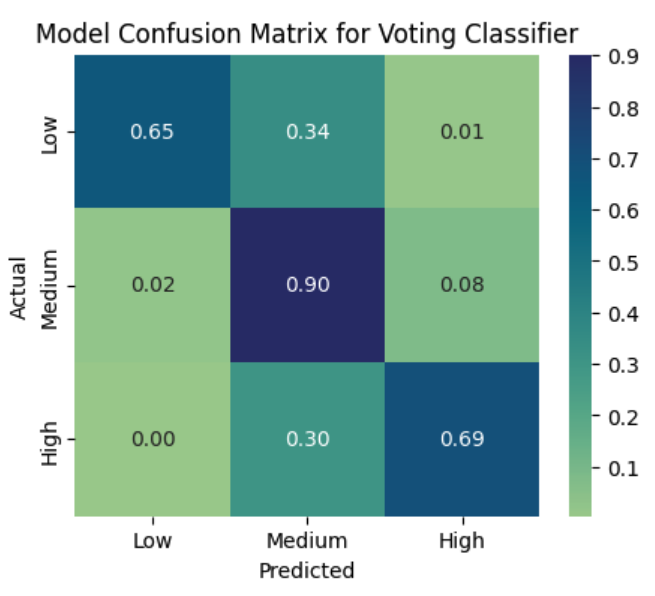
\includegraphics[scale=0.5]{matrix.png}
            \label{fig:matrix}
\end{figure}




\section{Data Insights}
The training data set is unbalanced, which causes all models to suffer on the least represented prediction.
The normalized confusion matrix for even the best models shows that \texttt{damage\_grade=1} has a recall\_ score close to 0.5, whereas \texttt{damage\_grade=2} had \texttt{recall\_score}s in the 0.8s.
Our efforts to improve the training data set, such as using the Synthetic Minority Oversampling Technique (SMOTE) to over sample the least represented label, did not noticeably improve submission scores.
Additionally, analyzing the feature importance to the labels predicted. We found that only the top 4 features really had a significant impact in accurately classifying the damage grade.

\section{Results}

The F1 score reached on the first 3 models was significantly lower than the baseline we got from the advanced models. So we didn't proceed further on tuning hyper-parameters and focused on the other models (resulting in the N/A in Table 1).
Very early in the approach our team decided to focus our efforts on XGBoost with the understanding it had the best ability to provide the highest score. Using XGBoost as the basis for the voting ensemble, using AutoML developed  8 independently trained XGBoost sub-models, where each sub-model had hyper-parameters tuned separately.
Weighting was tuned after each sub-model was completed. The final and best F1 score reached was 0.7528. See Table \ref{table:1}

\begin{table}
  \caption{Model F1 Scores}
  \label{table:1}
  \centering
  \begin{tabular}{llll}
    \toprule
    \multicolumn{2}{c}{}                   \\
    Model Name     & Training Set & Validation Set & Test Set (Submission) \\
    \midrule
    Multinomial Logistic Regression & 0.5662 & N/A & N/A    \\
    SVM & 0.5689 & N/A & N/A      \\
    Nearest Neighbor Classification       & 0.6353 & N/A & N/A \\
    CatBoost      & 0.7049 & 0.7289 & 0.7297 \\
    LightGBM      & 0.7915 & 0.7410 & 0.7394 \\
    XGBoost      & 0.7903 & 0.7507 & 0.7411  \\
    Voting Ensemble      & 0.7903 & 0.7507 & 0.7528  \\
    \bottomrule
  \end{tabular}
\end{table}

\section{Lessons Learned}

From our experience training a machine learning model, we learned that hyperparameter tuning can significantly improve submission scores, sometimes by as much as 0.1 micro-averaged F1 score.
We were able to achieve F1 score improvements for almost every base model we used by tuning the hyperparameters.
Ensemble stacking also helped to increase submission scores, although the improvement was usually modest after hyperparameter tuning. 

Training models on a CPU can be time-consuming, and using a GPU can significantly reduce the training time.
This is especially important considering that XGBoost is a processing-intensive model, and using a faster training model like LightGBM would have been more efficient.
If our team had more time, we would have thoroughly implemented LightGBM to optimize training time and model performance. 

We also discovered that hyperparameter tuning is time-consuming due to cross-validation, and running the algorithm on all features, especially those that don't provide much prediction information.
This does not just lead to longer processing time but can also lead to overfitting. We would have liked to explore dimension reduction techniques like PCA to help speed up the training algorithms.
We also found that different models resulted in a different set of best features for predicting labels, indicating the importance of having domain knowledge to identify relevant features. 

In addition, we learned that multi-classification using this dataset did not yield the best accuracy, and that combining output labels to create a binomial classification problem could improve F1 scores.
We also discovered that many ML models have built-in features that can handle missing data entries, enable categorical features, and use one-hot encoding. 

Finally, we realized that the more complex models we used, the harder it was to understand how they made predictions, highlighting the black box nature of machine learning.
While these models could make good predictions, we couldn't pinpoint which specific features and weighting were used to calculate the damage for a specific building.

\section*{References}

{
\small

[1] https://medium.com/analytics-vidhya/richters-predictor-modeling-earthquake-damage-b44e3dbdaef

[2] Learing to tune xgboost's hyperparameters https://www.analyticsvidhya.com/blog/2016/03/complete-guide-parameter-tuning-xgboost-with-codes-python/

[3] How to build an CatBoost model: https://catboost.ai/en/docs/concepts/tutorials

[4] How to build an XGBoost model: https://xgboost.readthedocs.io/

[5] How to build a LightGBM model: https://lightgbm.readthedocs.io/

[6] A Python library that helps with hyperparamter tuning: https://optuna.readthedocs.io/

[7] Azure AutoML: https://learn.microsoft.com/en-us/azure/machine-learning/concept-automated\\-ml?view=azureml-api-2

[8] The blog post that helped us get started: https://drivendata.co/blog/richters-predictor-benchmark/

}

\end{document}
